\documentclass[12pt,a4paper,twoside,twocolumn]{article}
\usepackage{style}

\author{Ludovic}
\title{Des figures pour \LaTeX}
\begin{document}
\maketitle

%\newcommand*{\CommonPath}{\currfiledir}% 

\section{Données}

\section{Figures}
\blindtext[10]

\begin{figure*} % Le * implique si il y a des colonnes,  la figure occupe quand mm toute la largeur.
  \begin{center}
    \frame{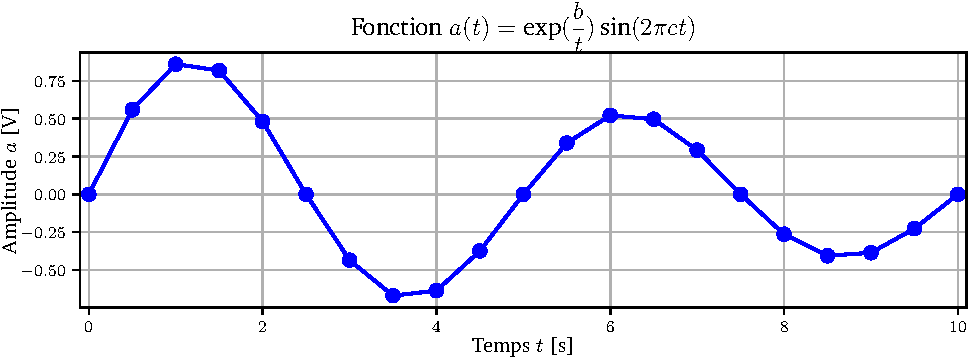
\includegraphics[width = \textwidth]{data/fig_python}}
    \caption{La grande figure.}
  \end{center}
\end{figure*}

% VERSION UNE COLONNE
\begin{figure} % Le * implique si il y a des colonnes,  la figure occupe quand mm toute la largeur.
  \begin{center}
    \frame{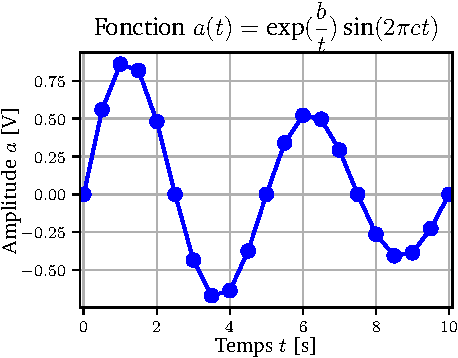
\includegraphics[width = \columnwidth]{data/fig_python_small}}
    \caption{La petite figure.}
  \end{center}
\end{figure}



\begin{figure}
\documentclass{standalone}
\usepackage{../style}

\begin{document}


\begin{tikzpicture} % Environnement pour faire un dessin avec Tikz
  \begin{axis}[
              xlabel = {Temps, $t$ [s]},
              ylabel = {Amplitude, $a$ [V]},
              title = {Fonction $a(t) = \exp(\frac{b}{t}) \sin(2\pi c t)$},
              width = \columnwidth,
              minor tick num = 4,
              ymin = -1.,
              ymax = 1.,
              xmin = 0.,
              ymax = 1.,
              axis x line = bottom,
              axis y line = left,]
    \addplot [
              color = blue,
              mark = o,
              line width = 1pt,
             ]
             table[x = x, 
                   y = y,
                   col sep = comma]{\currfiledir../data/data.csv};
  \legend{Data}
  \end{axis}	
\end{tikzpicture}
\end{document}
\caption{La petite figure avec PGFPlots.}
\end{figure}

\blindtext[10]

\end{document}